\begin{figure}[bh!]
    \vspace{-0.3em}
    \centering
    \begin{subfigure}{\textwidth}
        \centering
        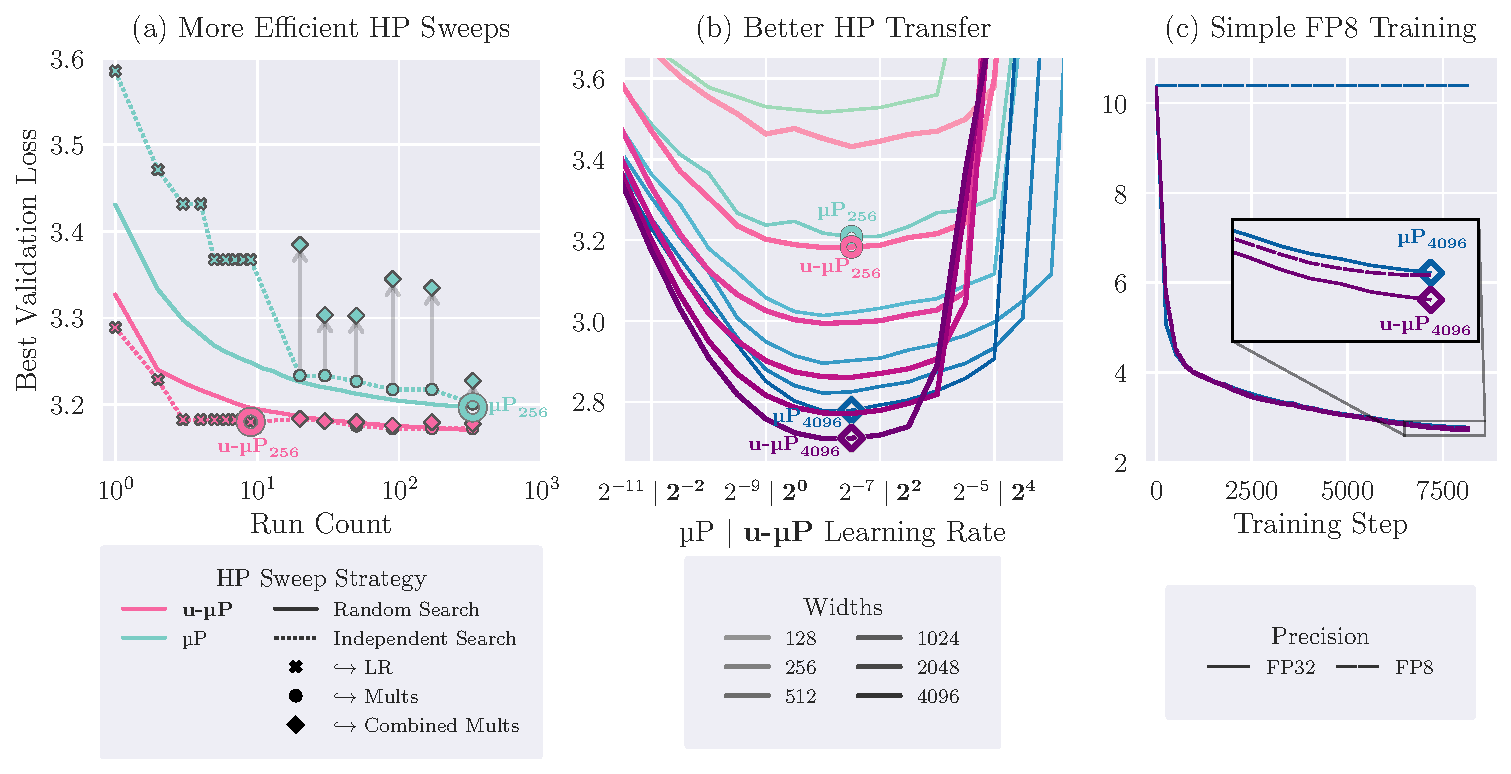
\includegraphics[width=\textwidth]{arXiv/figures/fig1_combined_v3.2.pdf}
    \end{subfigure}
    \caption{\textbf{(a)} Two different HP sweeping processes used for \mup\ and \umup\ proxy models. Unlike \mup, \umup\ admits independent (1D) search due to careful HP design. The first part of independent search is an LR sweep, which alone reaches near-optimal loss for \umup. \textbf{(b)} Using the best proxy HPs from (a), we train many models at different widths and LRs. The best LR for width 256 is \char`\~ optimal for 4096, showing LR transfer along with lower loss. \textbf{(c)} We re-train with a simple un-scaled {\texttt{.to(float8)}} cast on matmul inputs. This would fail for other models, but \umup\ trains with minimal degradation.}
    \label{fig:fig1}
    \vspace{-0.7em}
\end{figure}

\section{Introduction} \label{sec:introduction}

The challenges of large-model training extend beyond the domain of engineering; they are also \mbox{\textit{algorithmic}} in nature. Effective approaches for training smaller models are not guaranteed to work at the multi-billion-parameter scale used for today's large language models (LLMs). These difficulties can be framed in terms of stability, which we consider in three forms: 

\begin{enumerate}
    \item feature learning stability, which ensures that parts of the model do not learn too fast or slow relative to each other. 
    \item hyperparameter stability, which ensures that the optimal HPs for small models remain unchanged as the model size grows.
    \item numerical stability, which ensures that floating-point representations during training stay within the range of a given number format.
\end{enumerate}

% The standard approach to large-model training suffers from these stability issues. The logbooks of recent LLM training efforts reflect this \citep{BLOOM_chronicles, OPT_logbook, Flamingo_memo, Bloomberg_GPT}, with speculative manual adjustments made throughout training to fix spikes and plateaus in the loss, some of which can be attributed to problems of stability. A simple solution to these challenges promises to make large-model training easier and more cost-efficient.

The Maximal Update Parametrization (\mup)~\citep{Tensor_Programs_IV,Tensor_Programs_V} targets the first two sources of instability. \mup\ defines a set of scaling rules that in principle make a model's optimal HP values consistent across model sizes and ensure `maximal feature learning' in the infinite-width limit. The practical benefits of this are that models continue to improve as they get larger, and that practitioners can re-use a set of HP values (especially the learning rate) found for a small \textit{proxy} version of their model, on a larger \textit{target} model. This is vital for modern LLM training, where the cost of sweeping over candidate HP values for the target model is prohibitive. Consequently, \mup\ has been adopted by several open LLM training efforts \citep{Cerebras_GPT, BTLM, LLM360, MiniCPM} and there are indications of its use in state-of-the-art LLMs\footnotemark.

\footnotetext{The GPT-4 technical report~\citep{GPT4} hints at the use of \mup\ by including \citep{Tensor_Programs_V} in its references, without citing it directly. The multipliers present in the Grok~\citep{Grok} codebase also suggest the use of \mup.}

However, there exists a gap between the extensive theory underpinning \mup\ and its effective use in practice. This relates to issues surrounding efficient HP search, HP transfer, interpretability, ease-of-use and low-precision training. Some of these problems have been observed in the literature \citep{Exploration_Of_Mu_Transfer, Falcon, Tensor_Programs_V}; others we outline here for the first time. As a result, \mup\ does not necessarily provide the kind of simple, stable scaling for which a user might hope. 

To address this, we propose the Unit-Scaled Maximal Update Parametrization (\umup). \umup\ combines \mup\ with another closely-related training innovation, Unit Scaling \citep{Unit_Scaling}. \mup\ ideally provides consistent training dynamics across model sizes, but says little about what those dynamics should be. Unit Scaling addresses this by proposing an ideal principle for dynamics: unit variance for all activations, weights and gradients. Unit Scaling was initially designed to ensure stable numerics, but in the context of \mup\ the principle of unit-scale brings many additional benefits. We show that it provides a foundation upon which the broader range of drawbacks identified for \mup\ can be addressed.

\subsection{Contributions} \label{sec:introduction:contributions}

% Our resulting \umup\ method can be seen as an improved version of \mup, which 
We focus on LLMs in this work as this is the domain where \mup\ has primarily been used in the literature (though \umup's principles should extend to other architectures). We contribute the following:

\begin{enumerate}
    \item \textbf{Drawbacks of standard \mup:} We show that the way \mup\ is typically applied has several limitations, and does not give effective transfer for Llama-style models (\Cref{sec:the_challenges_with_mup_in_practice}).

    \item \textbf{Simpler scaling rules:} \umup\ is easier to implement in practice than \mup, and removes the unnecessary `base shape' and initialization-scale HPs (\Cref{{sec:umup:combining_mup_with_us}}; \Cref{table:mup_umup_schemes}).

    \item \textbf{Out-of-the-box FP8 training:} \umup\ models generate tensors that lie close to the center of a floating point format's range, meaning that most matrix multiplications can be performed in FP8 via a simple \texttt{.to(float8)} cast without dynamic rescaling.

    \item \textbf{A principled, interpretable \& independent set of HPs:} The set of transferable HPs used in the \mup\ literature is chosen in an inconsistent and arbitrary way. We provide concrete recommendations for a good set of transferable HPs to use with \umup\ (\Cref{sec:umup:principled_hps}).

    \item \textbf{Improved HP transfer:} We identify a problem with the scaling of the embedding layer's LR under \mup. Fixing this for \umup\ gives us better scaling with width (\Cref{sec:umup:emb_lr_rule}).

    \item \textbf{A more efficient approach to HP search:} We show that \umup\ facilitates a cheaper independent search method, attaining near-optimal loss when only sweeping the LR (\Cref{sec:umup_hp_search}).
\end{enumerate}

We provide a guide for using \umup\ in \Cref{app:using_umup_guide}, and a library \citep{us_library} implementing \umup\ functions, layers and optimizers, outlined in \Cref{app:us_lib_guide}.
